\documentclass[12pt,a4paper,oneside]{report}

\usepackage[margin=1in,headheight=15pt]{geometry}
\usepackage[T1]{fontenc}
\usepackage[utf8]{inputenc}
\usepackage{lmodern}
\usepackage{microtype}
\usepackage{graphicx}
\usepackage{booktabs}
\usepackage{tabularx}
\usepackage{longtable}
\usepackage{array}
\usepackage{enumitem}
\usepackage{listings}
\usepackage{caption}
\usepackage{subcaption}
\usepackage{pdflscape}
\usepackage{tikz}
\usetikzlibrary{arrows.meta,positioning,shapes.geometric,fit,backgrounds}
\usepackage{fancyhdr}
\usepackage{titlesec}
\usepackage{xcolor}
\usepackage{hyperref}

\definecolor{nationgreen}{HTML}{006A4E}
\definecolor{nationdark}{HTML}{062D27}
\definecolor{nationred}{HTML}{F42A41}
\definecolor{nationmint}{HTML}{38D6A2}
\definecolor{softgreen}{HTML}{EAF5F1}
\definecolor{softgray}{HTML}{F4F6F7}
\definecolor{riskred}{HTML}{A61B29}
\definecolor{riskamber}{HTML}{9A6700}
\definecolor{ink}{HTML}{17252A}

\hypersetup{
  colorlinks=true,
  linkcolor=nationgreen,
  urlcolor=nationgreen,
  citecolor=nationgreen,
  pdftitle={NationX Full Project Analysis and Technical Report},
  pdfauthor={SELECT * FROM WINNERS},
  pdfsubject={Software Engineering and DBMS Project Report}
}

\graphicspath{{assets/}{../../}}
\setlength{\parindent}{0pt}
\setlength{\parskip}{0.65em}
\setlength{\emergencystretch}{2em}
\setlist{nosep,leftmargin=1.5em}
\renewcommand{\arraystretch}{1.18}

\pagestyle{fancy}
\fancyhf{}
\fancyhead[L]{\textcolor{nationgreen}{NationX}}
\fancyhead[R]{Full Project Analysis}
\fancyfoot[C]{\thepage}
\renewcommand{\headrulewidth}{0.4pt}

\titleformat{\chapter}[display]
  {\normalfont\bfseries\color{nationdark}}
  {\filleft\Large\chaptername\ \thechapter}
  {0.5ex}
  {\titlerule\vspace{1ex}\Huge}
\titleformat{\section}{\Large\bfseries\color{nationgreen}}{\thesection}{0.75em}{}
\titleformat{\subsection}{\large\bfseries\color{nationdark}}{\thesubsection}{0.75em}{}

\lstdefinestyle{nationcode}{
  basicstyle=\ttfamily\small,
  backgroundcolor=\color{softgray},
  frame=single,
  rulecolor=\color{nationgreen!35},
  breaklines=true,
  showstringspaces=false,
  keywordstyle=\color{nationgreen}\bfseries,
  commentstyle=\color{gray},
  stringstyle=\color{riskred},
  numbers=left,
  numberstyle=\tiny\color{gray},
  xleftmargin=1.5em,
  framexleftmargin=1em
}
\lstset{style=nationcode}

\newcommand{\statusgood}{\textcolor{nationgreen}{\textbf{Verified}}}
\newcommand{\statuswarn}{\textcolor{riskamber}{\textbf{Partial / conditional}}}
\newcommand{\statusrisk}{\textcolor{riskred}{\textbf{Open risk}}}
\newcommand{\code}[1]{\texttt{#1}}
\newcommand{\projectmetric}[2]{%
  \begin{minipage}[t]{0.22\textwidth}\centering
  {\Large\bfseries\color{nationgreen}#1}\par
  {\small #2}
  \end{minipage}}

\begin{document}

\begin{titlepage}
\begin{tikzpicture}[remember picture,overlay]
  \fill[nationdark] (current page.south west) rectangle (current page.north east);
  \fill[nationgreen] (current page.south west) rectangle ([xshift=1.3cm]current page.north west);
  \fill[nationred] ([xshift=-4.0cm,yshift=-3.6cm]current page.north east) circle (1.15cm);
  \draw[nationmint!30,line width=1.5pt] ([xshift=1.8cm,yshift=2.1cm]current page.south west)
    -- ([xshift=-1.5cm,yshift=2.1cm]current page.south east);
\end{tikzpicture}

\vspace*{2.0cm}
{\color{nationmint}\Large SOFTWARE ENGINEERING AND DBMS PROJECT\par}
\vspace{0.7cm}
{\color{white}\fontsize{42}{48}\selectfont\bfseries NationX\par}
\vspace{0.3cm}
{\color{white}\Huge Bangladesh, Connected.\par}
\vspace{1.2cm}
{\color{white!85}\LARGE Full Project Analysis and Technical Report\par}

\vfill
\begin{tabular}{@{}ll@{}}
\color{nationmint}\textbf{Project type} & \color{white}Central government services portal (academic demonstration)\\
\color{nationmint}\textbf{Team} & \color{white}\texttt{SELECT * FROM WINNERS}\\
\color{nationmint}\textbf{Primary stack} & \color{white}React, Express, MySQL/MariaDB\\
\color{nationmint}\textbf{Analysis date} & \color{white}1 October 2026\\
\color{nationmint}\textbf{Evidence base} & \color{white}Source code, SQL, documentation, live local build and tests\\
\end{tabular}
\vspace{2.7cm}

{\color{white!65}\small This report evaluates the repository as inspected. NationX is not an official
government service and is not approved for public deployment or real citizen data.\par}
\end{titlepage}

\pagenumbering{roman}
\chapter*{Abstract}
\addcontentsline{toc}{chapter}{Abstract}

NationX is a broad, locally hosted academic e-government portal modeled on Bangladesh's
public-service environment. It integrates identity, passport, health, water, tax, land,
agriculture, education, admissions, community, commerce, reporting, and administration
within one application. The current repository is substantially more mature than its original
static implementation: it contains a React 19 interface alongside the retained legacy frontend,
an Express 5 REST backend, a large MySQL/MariaDB data model, role-scoped administration,
an applicant-specific NID workflow, a bilingual citizen guide, locally trained and fine-tuned
AI/ML services, medicine-image transcription, n8n event automation, database installers and
migrations, and several layers of automated tests. Its medicine knowledge pipeline processes a
nearly 60,000-record source dataset into a normalized catalogue of 53,987 canonical medicines.

The strongest part of the project is its breadth and database-centered workflow modeling. The
source currently defines 413 route handlers across the main route and assistant modules and 176
\code{CREATE TABLE} occurrences across 38 SQL files; duplication and migration order mean that
these figures must not be confused with the installed object count. The inspected development
database contained 156 base tables, 17 views, and 16 triggers, while the baseline test database
contained 131 base tables, 17 views, and 16 triggers. Stored routines are intentionally deferred
on the observed XAMPP MariaDB host because its \code{mysql.proc} system-table layout is
incompatible.

The project is suitable for a controlled course demonstration with synthetic data. It is not
production-ready. The principal blockers are unauthenticated or over-broad personal-data lookup,
unverified payment callbacks, public upload storage, permissive CORS, browser-local token storage,
incomplete workflow transition enforcement, schema drift, and a currently incomplete medicine
migration in the test database. The report proposes a staged path from demo reliability to a
secure deployable architecture without discarding the project's educational strengths.

\chapter*{Report Scope and Method}
\addcontentsline{toc}{chapter}{Report Scope and Method}

This is a repository-level technical assessment, not a restatement of the older documentation.
Evidence was gathered from the current application entry point, route definitions, controllers,
middleware, React components, legacy assets, SQL schemas and migrations, scripts, tests, security
tracker, migration matrix, and live local execution. Static counts are reported as source
occurrences; installed database counts are reported separately. Fresh screenshots were captured
from the local React build using the synthetic citizen and administrator accounts.
Descriptions of the local-model deployment and n8n automation layer also incorporate architecture
details supplied by the project team; their model weights, training runs, and n8n workflow exports
are deployment artifacts rather than files contained in this repository snapshot.

The following verification was run during preparation:

\begin{itemize}
  \item React production build: \statusgood.
  \item React component and contract suite: \statusgood, 25 files and 154 tests passed.
  \item Backend regression run: 53 checks passed before two medicine tests failed because the
        test database lacked \code{medicine\_import\_batches} and
        \code{medicine\_scan\_sessions}; five later files were cancelled when the stalled run was
        stopped. This is recorded as a current environment/migration defect, not as an application-wide pass.
  \item Local authenticated rendering: citizen dashboard and administrator workspace loaded
        successfully against the current backend and database.
\end{itemize}

\tableofcontents
\listoffigures
\listoftables
\clearpage
\pagenumbering{arabic}

\chapter{Project Overview}

\section{Problem statement}

Public services are typically divided among departments, each with its own forms, identifiers,
offices, status vocabulary, and approval process. NationX explores a unified digital front door in
which a citizen authenticates once, reaches several service domains, submits requests, follows
their status, and receives notifications. Administrators work in separately authenticated,
domain-scoped queues. The design is intentionally broad because its academic objective is to
demonstrate relational modeling, constraints, triggers, views, stored routines, APIs, and user
interfaces across a realistic multi-domain system.

\section{Current project snapshot}

\begin{center}
\projectmetric{413}{source route handlers}\hfill
\projectmetric{156}{base tables in dev DB}\hfill
\projectmetric{17}{installed views}\hfill
\projectmetric{154}{passing React tests}
\end{center}

\vspace{1em}

\begin{table}[htbp]
\centering
\caption{Repository snapshot from the inspected working tree}
\label{tab:snapshot}
\begin{tabularx}{\textwidth}{>{\bfseries}l r X}
\toprule
Item & Observed value & Interpretation\\
\midrule
Application code & about 89,050 lines & JS, JSX, SQL, Python, HTML, and CSS in the principal source trees\\
API route handlers & 413 & Static count of Express router definitions for the five HTTP methods\\
SQL files & 38 & Schemas, views, triggers, procedures, migrations, and seeds\\
SQL table declarations & 176 & Includes repeated/replacement definitions; not an installed-table count\\
Development database & 156 tables, 17 views, 16 triggers & Live local observation on 1 October 2026\\
Test database & 131 tables, 17 views, 16 triggers & Missing medicine catalogue/scan tables at verification time\\
Frontend pages & 29 routed React experiences & Original \code{.html} URL contracts preserved by React Router\\
Legacy frontend & 30 HTML files & Deliberately retained as rollback/reference implementation\\
React tests & 25 files, 154 tests & All passed in the current verification run\\
Medicine dataset & 57,799 source records & Normalized into 53,987 canonical medicines with field-level provenance\\
Committed upload files & 41 files & Privacy concern; content must be audited and removed before publication\\
\bottomrule
\end{tabularx}
\end{table}

\section{Stakeholders and actors}

\begin{table}[htbp]
\centering
\caption{Principal system actors}
\begin{tabularx}{\textwidth}{>{\bfseries}p{0.22\textwidth} X X}
\toprule
Actor & Primary goals & Current control boundary\\
\midrule
Citizen & Access records, submit applications, track services, manage profile and documents & Citizen JWT linked to \code{reg\_info}; ownership checks vary by endpoint\\
First-time NID applicant & Apply without an existing citizen NID identity & Separate UUID-based applicant identity and dedicated route boundary\\
Domain administrator & Review and update one service domain & Approved admin JWT plus active domain assignment\\
Divisional administrator & Work only within one domain and geographic division & Domain and division filters in scoped work queues\\
Platform administrator & Manage cross-domain work, roles, analytics, and access & \code{SUPER\_ADMIN} assignment\\
Automation runtime & Trigger workflows, weather, payment, email, local inference & n8n coordinates events while core authorization and data remain in Express and MySQL\\
Academic evaluator & Inspect database features, integration, and usability & Synthetic local dataset and demonstration workflows\\
\bottomrule
\end{tabularx}
\end{table}

\section{Functional coverage}

The citizen application covers authentication, profile and documents, a dashboard, history,
notifications, to-do management, and service modules for NID, passport, health, water, tax, land,
agriculture, education, admissions, stipends, community, market, shop, and contact. The
administration surface provides NID, passport, health, water, national reporting, access
assignment, audit views, and scoped work queues. Newer specialist features include first-time NID
applicant accounts, a bilingual service guide with optional voice input, and a medicine identifier
that transcribes visible package or prescription text and searches a normalized catalogue.

\chapter{Architecture and Technology}

\section{Logical architecture}

\begin{figure}[htbp]
\centering
\resizebox{\textwidth}{!}{%
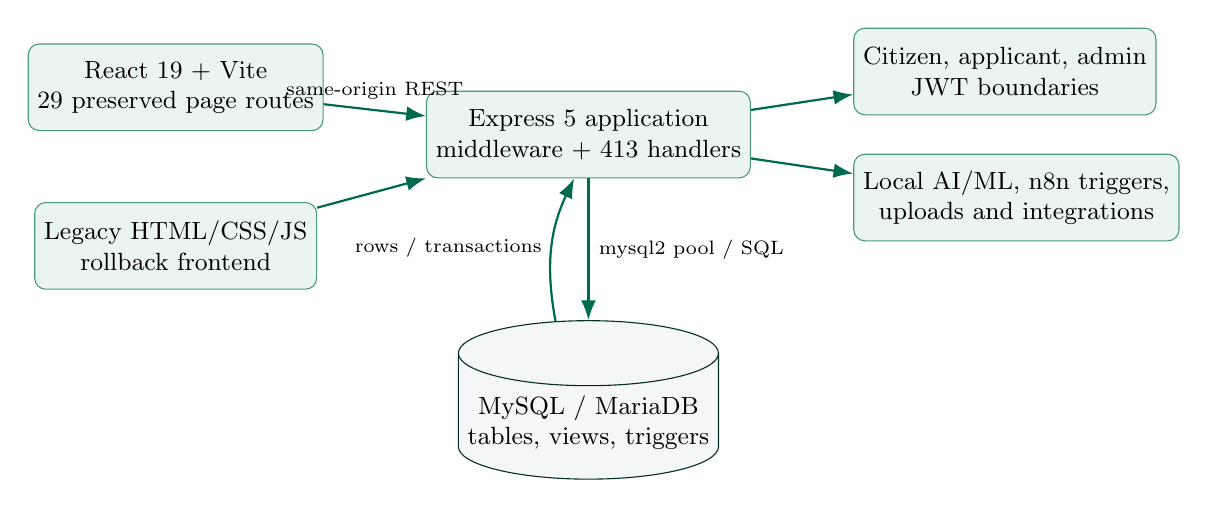
\begin{tikzpicture}[
  node distance=9mm and 13mm,
  box/.style={draw=nationgreen!70,rounded corners,fill=softgreen,minimum width=3.5cm,minimum height=1.1cm,align=center,font=\small},
  store/.style={draw=nationdark,shape=cylinder,shape border rotate=90,aspect=.25,fill=softgray,minimum width=3.0cm,minimum height=1.2cm,align=center,font=\small},
  arrow/.style={-{Latex[length=2.5mm]},thick,draw=nationgreen}
]
\node[box] (react) {React 19 + Vite\\29 preserved page routes};
\node[box,below=of react] (legacy) {Legacy HTML/CSS/JS\\rollback frontend};
\node[box,right=of react,yshift=-6mm] (express) {Express 5 application\\middleware + 413 handlers};
\node[box,right=of express,yshift=8mm] (auth) {Citizen, applicant, admin\\JWT boundaries};
\node[box,right=of express,yshift=-8mm] (services) {Local AI/ML, n8n triggers,\\uploads and integrations};
\node[store,below=18mm of express] (mysql) {MySQL / MariaDB\\tables, views, triggers};
\draw[arrow] (react) -- node[above,font=\scriptsize]{same-origin REST} (express);
\draw[arrow] (legacy) -- (express);
\draw[arrow] (express) -- (auth);
\draw[arrow] (express) -- (services);
\draw[arrow] (express) -- node[right,font=\scriptsize]{mysql2 pool / SQL} (mysql);
\draw[arrow,bend left=18] (mysql) to node[left,font=\scriptsize]{rows / transactions} (express);
\end{tikzpicture}
}
\caption{NationX logical architecture reconstructed from the current source}
\label{fig:architecture}
\end{figure}

The React application never connects to the database directly. It issues relative HTTP requests
to Express, which owns authentication, authorization, validation, file handling, transactions,
and SQL. Express can serve either the original \code{public/} frontend or, when
\code{FRONTEND\_MODE=react} and \code{client/dist} exists, the React shell for the migrated URL
allowlist. This route-by-route cutover preserves bookmarks and callback paths while keeping a
rollback option.

\section{Technology assessment}

\begin{table}[htbp]
\centering
\caption{Technology stack and engineering implications}
\begin{tabularx}{\textwidth}{>{\bfseries}p{0.18\textwidth} p{0.28\textwidth} X}
\toprule
Layer & Technology & Assessment\\
\midrule
Frontend & React 19, React Router 7, Vite 8, Three.js & Modern component model, lazy-loaded feature pages, preserved legacy paths; main and Three.js chunks deserve continued size control\\
Backend & Node.js CommonJS, Express 5 & Direct and easy to demonstrate; large fat-route files increase coupling and audit cost\\
Database & MySQL/MariaDB, \code{mysql2/promise} pool of 10 & Rich relational model and transactions; compatibility-sensitive routines and repeated schema definitions create drift risk\\
Authentication & JWT, bcrypt and bcryptjs & Clear citizen/admin separation and new scope assignments; fallback secrets and localStorage require hardening\\
Files & Multer, local disk, some BLOB storage & Practical locally; public legacy uploads and weak content isolation are unsuitable for real identity documents\\
AI/voice & Locally trained domain models and fine-tuned local Whisper & Private inference keeps voice and service-intent processing within the local deployment boundary\\
Automation & n8n event-triggered workflows & Coordinates status events, notifications, reminders, and operational workflow triggers without coupling them to page logic\\
External services & Open-Meteo, NASA POWER, SSLCommerz sandbox, Nodemailer/Ethereal & Appropriate for demonstration; payment and email flows are not production assurance\\
Testing & Node test runner, Vitest, Testing Library, Playwright, Python unittest & Good breadth and real database coverage; no CI gate and current test schema drift remain gaps\\
\bottomrule
\end{tabularx}
\end{table}

\section{Runtime and request pipeline}

The entry point applies Helmet with a localhost-oriented Content Security Policy, unrestricted
CORS, JSON and form parsing, a global API limiter (default now 2,000 requests per 15 minutes), an
applicant boundary, API routers, static frontend delivery, and a final error handler. The database
pool waits for connections and caps concurrency at ten. Application-level crash handlers append
to \code{server\_crash.log} and exit on uncaught failures.

The overall pipeline is understandable, but three architectural observations matter:

\begin{enumerate}
  \item \textbf{Routes are the service layer.} SQL and workflow logic mostly live directly in
        route modules. This is consistent with the project style but makes reuse and focused unit
        testing harder.
  \item \textbf{Frontend mode is operational configuration.} The same server can expose a legacy
        or React presentation depending on an environment variable and build availability.
  \item \textbf{Middleware is not uniformly sufficient.} A page guard improves user experience,
        but only API-side authentication, ownership, scope, and transition checks protect data.
\end{enumerate}

\chapter{Frontend Analysis}

\section{React migration and URL compatibility}

The React application maps the original page names directly, including
\code{/dashboard.html}, \code{/nid.html}, \code{/passport.html}, and admin URLs. Citizen routes
are wrapped with \code{CitizenGuard}; admin pages use \code{AdminGuard}; admission catalogue and
application routes remain public by design. Large feature pages are loaded lazily, while landing,
registration, dashboard, profile, documents, history, events, contact, and market are eagerly
imported.

The migration strategy is one of the project's best engineering decisions. It reduces cutover
risk, avoids breaking saved URLs and payment return addresses, and permits comparisons with the
original frontend. The cost is duplication: approximately 47,674 lines remain in the legacy
public HTML/JS/CSS tree while the React source adds approximately 11,878 lines.

\begin{figure}[htbp]
\centering

\includegraphics[width=\textwidth,height=.78\textheight,keepaspectratio]{nationx-landing.png}
\caption{Current React landing experience captured from the local production build}
\label{fig:landing}
\end{figure}

\section{Citizen experience}

The dashboard provides a recognizable portal shell, status summary, eight major department
cards, and supporting navigation. The current visual language is coherent: dark Bangladesh green,
high-contrast cards, Bengali cultural motifs, and a consistent service taxonomy. The dashboard
also exposes a cross-service request modal and the compact citizen guide.

\begin{figure}[htbp]
\centering
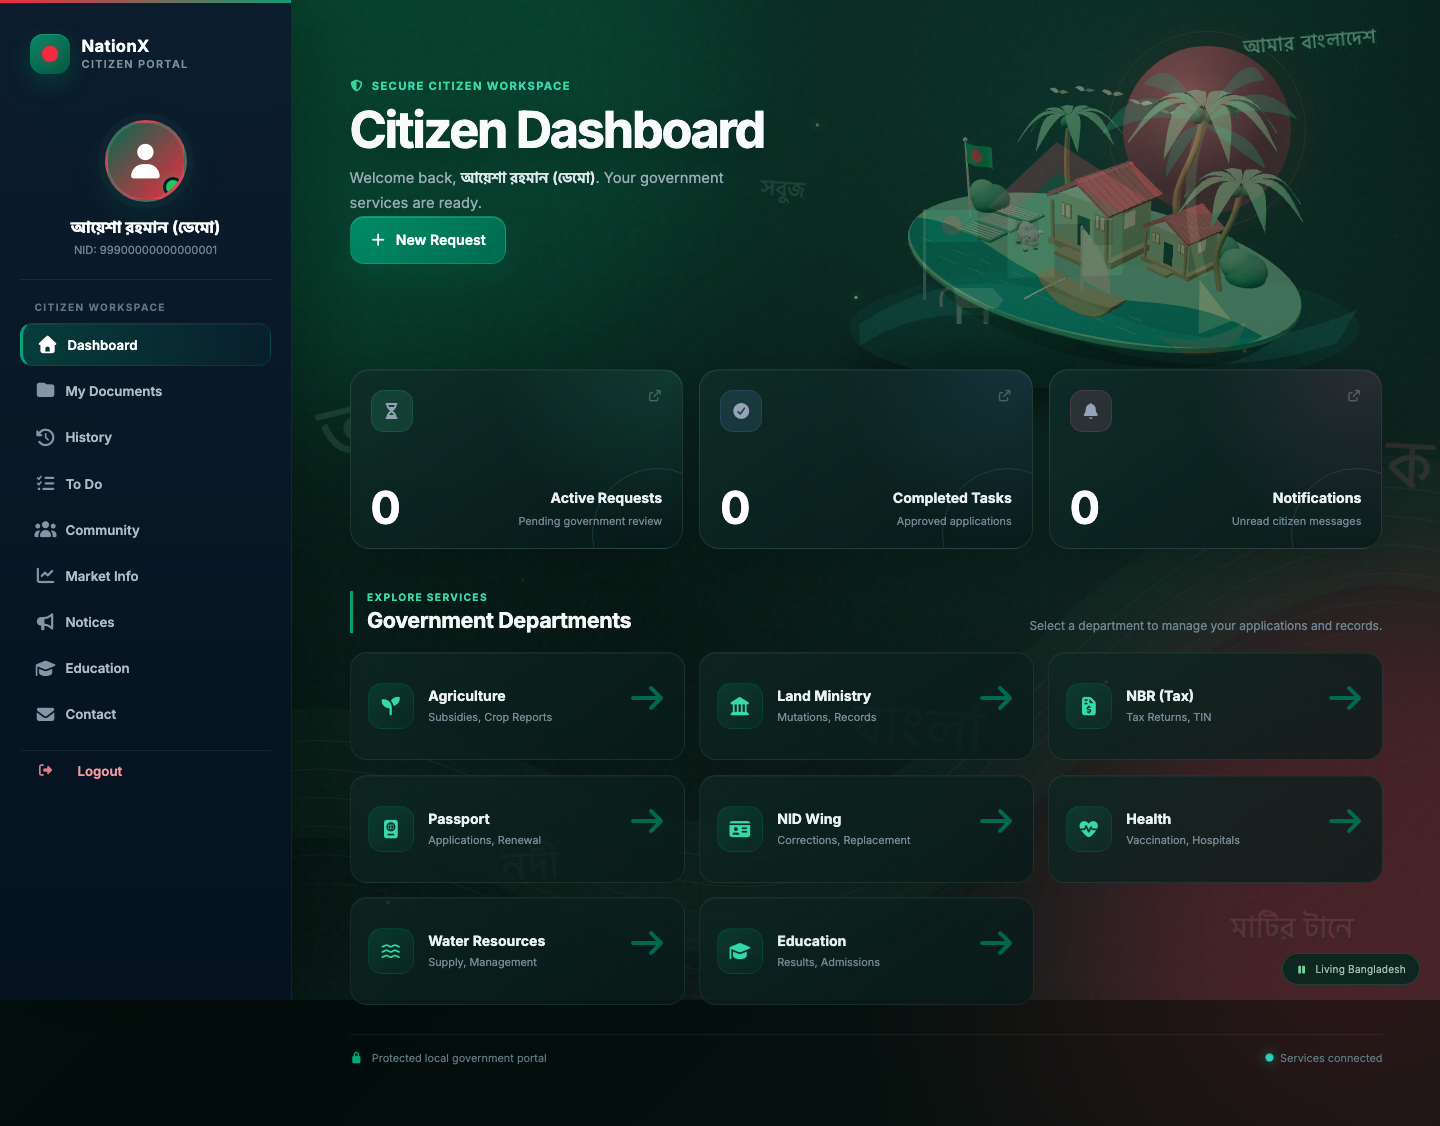
\includegraphics[width=\textwidth,height=.78\textheight,keepaspectratio]{nationx-dashboard.png}
\caption{Authenticated synthetic citizen dashboard}
\label{fig:dashboard}
\end{figure}

Strengths include preservation of server-side contracts, feature-level lazy loading, shared API
error handling, form submission locks, explicit payment-simulation labeling, and bilingual font
support. Accessibility and maintainability would benefit from a systematic audit of keyboard
order, focus restoration, color contrast, loading/error announcements, and shared form controls
across all 29 pages.

\section{Administrator experience}

The new administrator workspace represents responsibility as an explicit role and scope instead
of treating every approved administrator as globally privileged. It displays ten service domains,
the active jurisdiction, authorized queue, access assignments, audit navigation, and national
analytics. This is a meaningful improvement over a simple boolean \code{isAdmin} interface.

\begin{figure}[htbp]
\centering
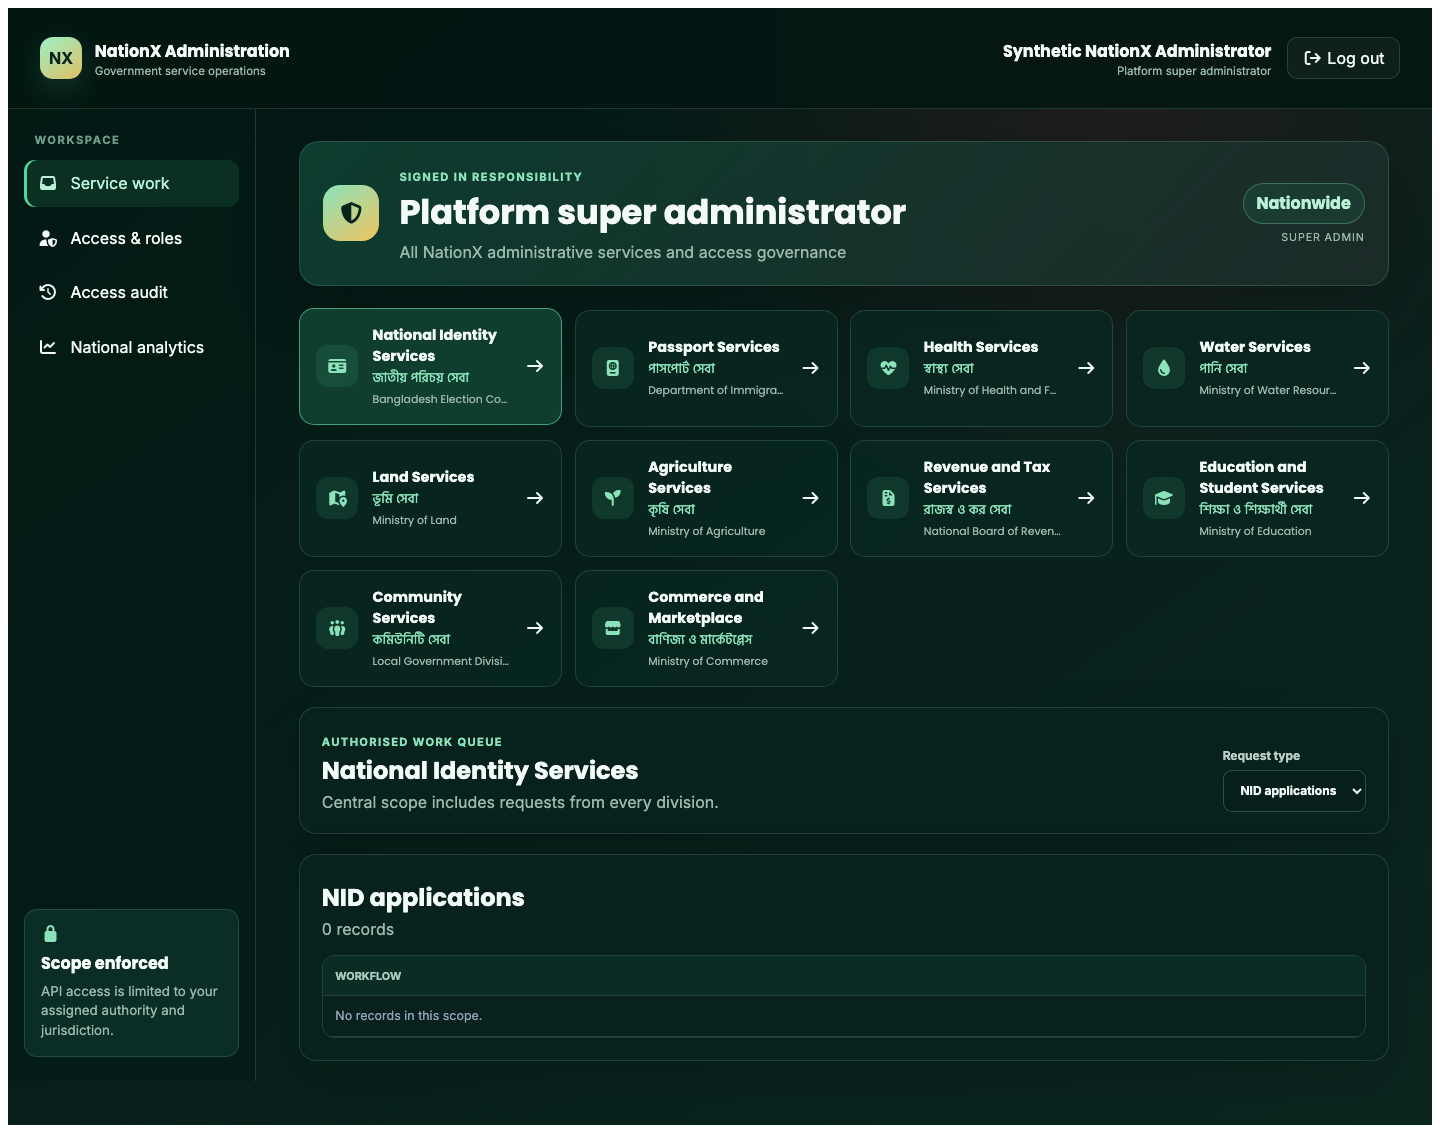
\includegraphics[width=\textwidth,height=.78\textheight,keepaspectratio]{nationx-admin-reports.png}
\caption{Authenticated platform-administrator workspace using synthetic data}
\label{fig:admin}
\end{figure}

The backend must remain authoritative: hiding cards is not authorization. The current
\code{adminMiddleware} reloads the administrator's status and assignment from the database for
each protected request, and domain/division helpers enforce the intended scope. Remaining admin
weaknesses include incomplete status-transition graphs, inconsistent unknown-ID behavior, limited
server-side pagination, and incomplete actor attribution in some trigger-generated history.

\section{Citizen guide and voice interaction}

The service guide supports Bengali and English text or voice, deterministic routing among 48
service destinations, 30 guided-form entries, and 33 authenticated status lookups. It reuses only
explicitly mapped blank profile fields, does not overwrite uploads or consent, and never submits
or pays automatically. Audio is limited to 15 seconds and sent to an authenticated endpoint for
transcription by a locally hosted, Bengali fine-tuned Whisper Medium model in quantized GGML
format. Speech remains within the local deployment boundary, and late transcription results are
discarded when the interaction closes.

This constrained design is preferable to a general autonomous chatbot for government forms. The
assistant helps the citizen operate the real form while retaining the form's validation and final
submission control. However, voice quality varies by device, and a language-model classification
result must never expand authorization or be treated as an approval decision.

\chapter{Backend and API Analysis}

\section{API scale and organization}

The current route surface is large. Table~\ref{tab:endpoints} reports source handler counts; it
does not claim that every endpoint is equally active or exposed in every frontend mode.

\begin{longtable}{@{}l r l r@{}}
\caption{Route handler definitions by module}\label{tab:endpoints}\\
\toprule
Module & Handlers & Module & Handlers\\
\midrule
\endfirsthead
\toprule
Module & Handlers & Module & Handlers\\
\midrule
\endhead
Admin core & 56 & Health & 40\\
NID & 33 & Water & 33\\
Agriculture & 30 & Department services & 29\\
Passport & 26 & Community & 18\\
Dashboard & 18 & Reports & 15\\
Tax & 14 & Shop & 13\\
University admission & 11 & Education & 5\\
Notice & 6 & Medicine catalogue & 4\\
Medicine scans & 7 & Authentication & 4\\
User profile & 3 & Payment & 3\\
Stipend & 3 & Contact & 1\\
Admin auth/access/work & 9 & Applicant routes & 8\\
First-time NID application & 14 & Assistant routes & 10\\
\midrule
\multicolumn{3}{r}{\textbf{Total source handler definitions}} & \textbf{413}\\
\bottomrule
\end{longtable}

The API breadth is impressive for a course project, but route count is not by itself a quality
measure. Several handlers repeat validation, authorization, SQL formatting, error mapping, and
pagination behavior. The largest module, \code{adminRoutes.js}, is about 1,753 lines. A safe
refactor should be incremental: extract shared validators and transaction helpers first, retain
route URLs and SQL semantics, and back each extraction with regression tests.

\section{Authentication and authorization}

Citizen login returns a one-hour JWT and records login activity. Admin login issues a separate JWT
with an admin claim; protected requests then reload current account status and an active role
assignment. The role model supports platform, domain, and division scopes across NID, passport,
health, water, land, agriculture, tax, education, community, and commerce.

The first-time NID applicant flow uses a different principal type and UUID. The global applicant
boundary prevents those tokens from entering legacy routes that interpret \code{id} as a numeric
\code{reg\_info.id}. This is a careful solution to identity confusion.

Known authentication risks are material:

\begin{itemize}
  \item citizen and admin code paths still contain fallback JWT secrets, and the citizen signing
        and verification fallbacks are historically inconsistent;
  \item tokens are stored in browser \code{localStorage}, raising the impact of any XSS flaw;
  \item unrestricted CORS is unsuitable for a deployed identity portal;
  \item some public or authenticated lookup endpoints return more personal data than necessary;
  \item several status mutations do not enforce a legal transition graph.
\end{itemize}

\section{Representative workflow: land mutation}

The land mutation path is one of the project's strongest end-to-end database examples. A citizen
submits a request linked to an ownership record. An authorized administrator begins a transaction
and selects the request. Approval updates status; the authoritative database trigger validates the
amount, locks/currently checks ownership, transfers all or part of the holding, rejects overdrawn
or ambiguous operations, and allows the application transaction to commit only if all effects
succeed. Regression tests cover full transfer, exact partial remainder, idempotency, concurrent
over-transfer prevention, invalid numeric values, and ambiguous service requests.

\begin{figure}[htbp]
\centering
\resizebox{\textwidth}{!}{%
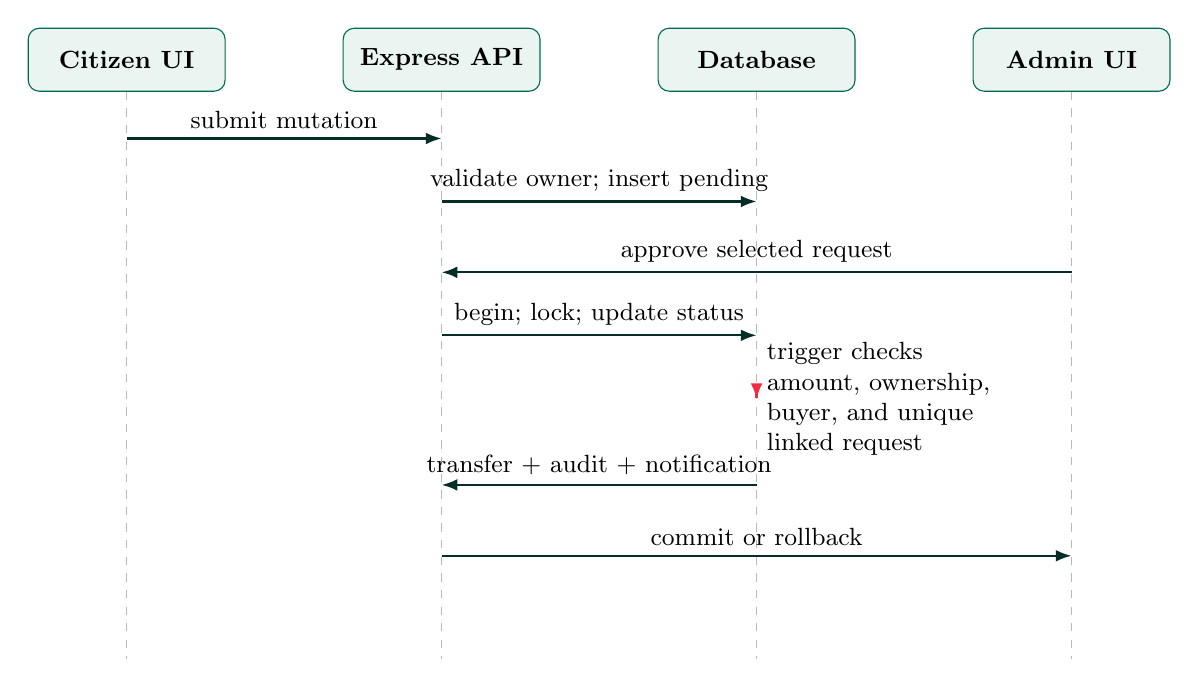
\begin{tikzpicture}[
  actor/.style={draw=nationgreen,rounded corners,fill=softgreen,minimum width=2.5cm,minimum height=.8cm,font=\small\bfseries},
  msg/.style={-{Latex[length=2mm]},draw=nationdark,thick},
  lifeline/.style={draw=gray!55,dashed},
  font=\small
]
\node[actor] (c) at (0,0) {Citizen UI};
\node[actor] (a) at (4,0) {Express API};
\node[actor] (d) at (8,0) {Database};
\node[actor] (m) at (12,0) {Admin UI};
\foreach \x in {c,a,d,m} \draw[lifeline] (\x.south) -- ++(0,-7.2);
\draw[msg] (c.south |- 0,-1) -- node[above]{submit mutation} (a.south |- 0,-1);
\draw[msg] (a.south |- 0,-1.8) -- node[above]{validate owner; insert pending} (d.south |- 0,-1.8);
\draw[msg] (m.south |- 0,-2.7) -- node[above]{approve selected request} (a.south |- 0,-2.7);
\draw[msg] (a.south |- 0,-3.5) -- node[above]{begin; lock; update status} (d.south |- 0,-3.5);
\draw[msg,draw=nationred] (d.south |- 0,-4.3) -- ++(0,-.01) node[right,text width=3.1cm]{trigger checks amount, ownership, buyer, and unique linked request};
\draw[msg] (d.south |- 0,-5.4) -- node[above]{transfer + audit + notification} (a.south |- 0,-5.4);
\draw[msg] (a.south |- 0,-6.3) -- node[above]{commit or rollback} (m.south |- 0,-6.3);
\end{tikzpicture}
}
\caption{Simplified land-mutation approval sequence}
\label{fig:land-sequence}
\end{figure}

\section{Payment behavior}

Payment functionality must be described precisely. The repository contains SSLCommerz sandbox
integration and clearly labeled React simulations, but multiple callbacks trust URL or client
values without signature, amount, ownership, or transaction-state validation. A simulation is
safe only because it intentionally performs no database write. Real land-tax, shop, passport,
water, and admission payment paths require a single verified callback architecture with server-side
order state, idempotency keys, amount/currency checks, gateway signature verification, and audit.

\chapter{Database Design and DBMS Features}

\section{Schema composition}

Database design is the centerpiece of NationX. The schema represents citizen identity,
administrative geography, NID, passport, health, water, tax, land, agriculture, education,
university admission, stipends, community, shopping, notifications, reporting, assistant state,
admin access, and medicine data. It uses primary and foreign keys, unique constraints, enums,
indexes, JSON fields where the shape is naturally variable, audit tables, views, triggers, and
procedural SQL.

The source has 176 table-creation statements, 23 view-creation statements, 19 trigger-creation
statements, and 25 procedure-creation statements. These are source occurrences across overlapping
files, not unique installed objects. The observed development database had 156 base tables, 17
views, and 16 triggers. The difference demonstrates why the installer and
\code{information\_schema} should be the authoritative basis for environment claims.

\begin{landscape}
\begin{figure}[p]
\centering

\includegraphics[width=.96\linewidth,height=.82\textheight,keepaspectratio]{nationx-er-overview.png}
\caption{Existing NationX complete ER diagram artifact (134-table project snapshot; use the high-resolution source for zoomed inspection)}
\label{fig:er}
\end{figure}
\end{landscape}

\section{Normalization and integrity}

The project includes \code{schema\_normalized.sql} to demonstrate 3NF/BCNF concepts, while domain
schemas contain practical denormalizations such as counters and status snapshots. Strong integrity
examples include foreign-key-bound ownership, unique tracking numbers, application state fields,
trigger-maintained counters, status history, and atomic land transfer.

There is also deliberate technical debt. Some older domains identify people inconsistently by
numeric user ID, NID string, email, or duplicated identity fields. Near-duplicate tables and
definitions occur across the master dump and domain files. The installer handles selected clashes
through reviewed transforms and ordered replacement, but this is fragile unless every schema
change is converted into a forward-only migration.

\section{Views, triggers, and routines}

The installed 17 views support consolidated profiles, service dashboards, education analysis,
inventory, reports, and other read models. Sixteen installed triggers perform tasks such as land
transfer authority, audit/history creation, denormalized like/comment counters, and cart/order
effects.

Approximately 25 procedure declarations exist in source, including processing, number generation,
tax calculation, eligibility checks, billing, and dashboard statistics. On the inspected XAMPP
MariaDB 10.4 environment, procedure installation is deferred because the host's
\code{mysql.proc} layout reflects an incomplete system-table upgrade. Active application code has
no required \code{CALL} sites, so the local demonstration can run, but the coursework claim should
say ``procedure catalogue present; runtime installation conditional'' rather than imply that all
routines are installed.

\section{Installer and migrations}

The installer allowlists only \code{central\_govt\_db} and \code{central\_govt\_db\_test}, refuses
automated development reset, strips database-selection statements, applies a controlled sequence,
uses synthetic hashed identities, checks required constraints and triggers, and validates the
baseline. These safeguards are excellent for an academic repository.

The migration chain is currently inconsistent with newer features. The installer applies
migration 008 (NID applicant/assistant) and 009 (admin roles), but does not install the medicine
catalogue and scan schemas from 006 and 007. Those are delegated to separate medicine scripts.
The test database used for this report lacked both medicine groups, which caused the regression
suite to fail. A single manifest should declare core, optional, and dataset-backed migrations,
and the test command should either provision required optional modules or skip them explicitly.

\chapter{AI-Assisted Features}

\section{Private local AI/ML architecture}

NationX uses a privacy-oriented local AI profile rather than depending on public generative-AI
services for its presentation deployment. The stack combines a locally trained, domain-constrained
intent model for government-service routing; a fine-tuned vision/OCR model for medicine labels and
prescriptions; and a locally hosted Bengali fine-tuned Whisper Medium model for speech recognition.
The models return schema-constrained results and remain advisory: ordinary validation,
authorization, database constraints, and human confirmation stay authoritative.

This architecture is particularly attractive for citizen services because sensitive voice,
identity, and health-related inputs can remain inside the controlled NationX environment. Local
deployment also improves demonstration reliability when internet access is unavailable and makes
the model version, inference settings, and retention policy controllable by the project team.

\section{Medicine identifier}

The medicine feature accepts a prescription or package image, validates and preprocesses it,
transcribes only visible medicine information through a structured schema, asks the user to
confirm/correct the result, searches a normalized catalogue, and may compare eligible alternatives
and estimated savings. Raw images are not intended to be persisted; session records keep hashes,
metadata, extracted items, candidates, confirmations, and estimates.

The underlying data pipeline combines 21,714 market rows and 36,085 registered-drug rows. After
validation and provenance-preserving normalization, these 57,799 source records produce 53,987
canonical medicine records, 74,989 medicine--ingredient relationships, 73,637 price observations,
36,082 registration records, and a 69,889-row flattened catalogue preview. The report therefore
describes this accurately as a \textbf{nearly 60,000-record medicine dataset}, rather than claiming
60,000 distinct canonical products. Every normalized value retains source links and review status.

Important safeguards in the source include prompt-injection resistance instructions, no patient
identity extraction, no diagnosis or treatment advice, nulls for unreadable values, explicit
professional-confirmation language, structured Zod validation, and eligibility flags separating
identification from price/savings comparisons. These controls are sensible, but they do not make
the feature medical advice. Every result must remain an aid for pharmacist/doctor confirmation.

\section{Local-model resilience}

The local inference layer separates image understanding, service-intent classification, and speech
recognition so that failure in one model does not disable ordinary forms or catalogue search. A
consecutive-failure circuit opens after three to five eligible transient failures, remains open for
a configured cooldown, and then probes the preferred local model again. Deterministic keyword
routing, manual service selection, catalogue lookup, and typed form entry remain available when a
model is unavailable. Model telemetry must contain only operational measurements and must not log
citizen speech, images, identifiers, or medical content.

\section{n8n event and trigger automation}

The automation tier uses n8n to connect application and database events with operational actions.
Its event-triggered workflows can coordinate application-status notifications, administrative
queue alerts, reminder schedules, escalation paths, and dataset-processing jobs while Express and
MySQL remain the systems of record. n8n does not approve requests or bypass authorization; it
reacts to validated events and invokes allowlisted internal actions with service credentials.

For production hardening, each workflow should be exported and version-controlled, signed webhook
requests should be verified, retries should be idempotent, credentials should stay in the n8n
secret store, and every automated action should carry a correlation ID into the audit log.

\section{Applicant assistant}

First-time NID applicants are modeled separately from registered citizens. Application drafts use
JSON fields with explicit versioning, private database-held documents, status history, expiring
confirmation tokens, and assistant event records. The separation prevents a person without an
issued NID from being treated as a fully registered citizen. This domain should retain explicit
wording that a NationX submission is a demonstration and is not government NID issuance.

\chapter{Quality Assurance and Verification}

\section{Test architecture}

\begin{table}[htbp]
\centering
\caption{Testing layers found in the repository}
\begin{tabularx}{\textwidth}{>{\bfseries}p{0.2\textwidth} p{0.25\textwidth} X}
\toprule
Layer & Tooling & Coverage examples\\
\midrule
Frontend unit/component & Vitest, Testing Library, jsdom & Guards, API client, forms, service pages, admin pages, voice hooks, guide behavior\\
Backend regression & Node test runner, real test DB & Ownership, role scope, status updates, SQL contracts, land concurrency, catalogue behavior\\
Browser journeys & Playwright/Chromium & Landing, citizen/admin login, routed pages, to-do lifecycle, medicine flow, guide workflow\\
Data pipeline & Python unittest and Node scripts & Medicine normalization, import, verification, and rollback\\
Build checks & Vite production build & Module transformation, route bundles, static asset references\\
\bottomrule
\end{tabularx}
\end{table}

\section{Current verification results}

\begin{table}[htbp]
\centering
\caption{Fresh verification performed for this report}
\begin{tabularx}{\textwidth}{>{\bfseries}p{0.26\textwidth} p{0.22\textwidth} X}
\toprule
Check & Result & Evidence / interpretation\\
\midrule
React production build & \statusgood & 115 modules transformed; build completed. Asset paths remain runtime-resolved. A chunk-size warning remains for Three.js.\\
React test suite & \statusgood & 25 files, 154 tests passed.\\
Authenticated citizen UI & \statusgood & Dashboard rendered against local Express and MySQL using the synthetic citizen.\\
Authenticated admin UI & \statusgood & Platform super-admin workspace rendered with role/scope data.\\
Backend regression suite & \statuswarn & 53 passed before two medicine tests failed; five later files were cancelled after a pending run was interrupted.\\
Medicine test schema & \statusrisk & Missing \code{medicine\_import\_batches} and \code{medicine\_scan\_sessions} in \code{central\_govt\_db\_test}.\\
Stored procedures & \statuswarn & Source catalogue exists; installation deferred by MariaDB system-table compatibility migration 005.\\
\bottomrule
\end{tabularx}
\end{table}

The older migration matrix records earlier successful runs (including 98 frontend tests, 71
backend checks, 11 medicine checks, and four Chromium journeys). Those are useful historical
evidence, but this report does not present them as the current result because the repository and
test counts have since changed.

\section{Observed build concerns}

The current Vite build reports that several \code{/images/*} CSS references remain unresolved at
build time and will be resolved at runtime. This is expected with Express serving \code{public/},
but it should be documented and covered by a production-mode smoke test. The generated Three.js
chunk is about 560 kB uncompressed and exceeds the default 500 kB warning threshold. Lazy-loading
the cinematic scene only on the landing experience already helps; further vendor splitting and
performance budgets would improve low-bandwidth access.

\chapter{Security, Privacy, and Reliability}

\section{Threat and risk summary}

\begin{longtable}{@{}p{0.19\textwidth} p{0.12\textwidth} p{0.57\textwidth}@{}}
\caption{Prioritized risk register}\label{tab:risks}\\
\toprule
Risk & Priority & Required treatment\\
\midrule
\endfirsthead
\toprule
Risk & Priority & Required treatment\\
\midrule
\endhead
Identity data disclosure & Critical & Authenticate and authorize every lookup, minimize fields, add consent/purpose controls, auditing, abuse limits, and isolated tests.\\
Unverified payment callbacks & Critical & Verify gateway signatures and server-side order state, match amount/currency/owner, use idempotency, and reject client-declared success.\\
Public/committed uploads & Critical & Remove real-looking documents, decide history cleanup, move uploads outside the web root, scan content, authorize downloads, and define retention.\\
Admission and education public lookup & Critical & Establish a publication policy; protect personal fields and guessable identifiers.\\
Agriculture contact exposure & Critical & Publish only approved listings and minimize contact data.\\
Fallback JWT secrets & High & Fail startup when a strong environment secret is absent; rotate and centralize secret configuration.\\
Browser token storage & High & Complete XSS review; prefer secure, HttpOnly, SameSite cookies where deployment architecture permits.\\
Permissive CORS & High & Use environment-specific origin, method, and header allowlists.\\
Dependency advisories & High & Review and upgrade in controlled batches; replace dependencies with unpatched transitive flaws.\\
Workflow transition gaps & High & Define server-side state machines and return 404/409 for invalid identifiers/transitions.\\
Schema drift & High & Adopt one migration manifest and generate schema documentation from installed metadata.\\
No CI/security gate & High & Run build, unit, DB regression, browser smoke, dependency audit, secret scan, and migration checks on every change.\\
\bottomrule
\end{longtable}

\section{Positive controls}

The security posture is not uniformly weak. Positive measures include Helmet and CSP, bcrypt
password hashing, parameterized SQL in many paths, upload size limits, citizen/admin/applicant
identity separation, current-admin database checks, domain/division authorization, ownership
regressions, transaction-backed land approval, allowlisted database targets, synthetic identities,
explicit payment simulation labels, and a detailed security tracker that avoids overstating
readiness.

\section{Reliability and operational gaps}

The crash handlers make failures visible locally but terminate the process; production would need
a supervisor, structured logs, correlation IDs, health/readiness endpoints, metrics, alerting, and
graceful shutdown of the HTTP server and database pool. Backups, point-in-time recovery, retention,
and disaster recovery are not established. Local-disk uploads are not horizontally scalable.

\chapter{Maintainability and Engineering Evaluation}

\section{Strengths}

\begin{itemize}
  \item unusually broad service-domain modeling with real relational relationships;
  \item genuine DBMS features rather than an ORM-only CRUD demonstration;
  \item backward-compatible React migration preserving original URLs;
  \item separate citizen, applicant, and scoped administrator identities;
  \item synthetic baseline and allowlisted installer safety;
  \item realistic regression tests for ownership, concurrency, and trigger authority;
  \item careful labeling of demonstration limits and unverified payments;
  \item culturally coherent, bilingual visual design.
\end{itemize}

\section{Weaknesses}

\begin{itemize}
  \item very large route modules combine HTTP, workflow, SQL, and response formatting;
  \item duplicate schema definitions and independent feature installers allow environment drift;
  \item authorization and input validation quality vary across older endpoints;
  \item legacy and React frontends double the maintenance surface;
  \item no formal API specification, CI pipeline, linting baseline, or coverage threshold;
  \item demo external integrations sit beside routes that resemble production success callbacks;
  \item historical uploads and broad personal-data responses create severe privacy exposure.
\end{itemize}

\section{Balanced maturity assessment}

\begin{table}[htbp]
\centering
\caption{Qualitative maturity scorecard}
\begin{tabularx}{\textwidth}{>{\bfseries}p{0.26\textwidth} p{0.16\textwidth} X}
\toprule
Area & Rating & Rationale\\
\midrule
Academic DBMS depth & Strong & Large multi-domain schema, views, triggers, procedure catalogue, complex queries\\
Functional breadth & Strong & Citizen, applicant, service, commerce, assistant, and admin experiences\\
User-interface quality & Strong for demo & Cohesive React design and preserved navigation contracts\\
Automated verification & Moderate--strong & Multiple test layers, but current DB migration drift and no CI gate\\
Maintainability & Moderate & Clear domain files but substantial fat-route and duplicated-frontend cost\\
Security/privacy & Weak for production & Several critical documented access, upload, and payment issues\\
Deployability & Local demo only & Environment-coupled database, sandbox services, no production operations model\\
Documentation honesty & Strong & README, trackers, matrices, and simulation labels state limitations clearly\\
\bottomrule
\end{tabularx}
\end{table}

\chapter{Recommendations and Roadmap}

\section{Priority 0: protect people and money}

Before any public deployment:

\begin{enumerate}
  \item remove sensitive uploads from the served tree and repository, decide whether Git history
        must be rewritten, and replace them with unmistakably synthetic fixtures;
  \item disable or protect public NID, admission, education, and agriculture endpoints that expose
        personal or contact data;
  \item block every database-writing payment-success path until a verified gateway callback module
        is implemented and tested;
  \item require a strong JWT secret at startup, define restricted CORS, and review token storage;
  \item add immutable, actor-aware audit records for identity access and administrative mutations.
\end{enumerate}

\section{Priority 1: make environments reproducible}

\begin{enumerate}
  \item create one migration registry that records dependencies and whether a module is core,
        optional, or dataset-backed;
  \item make \code{npm test} provision or validate the complete schema it expects, including
        medicine migrations 006 and 007;
  \item add a non-destructive \code{db:status} command reporting version, installed migrations,
        missing objects, routine compatibility, and seed identity counts;
  \item run the installer against supported MySQL and MariaDB versions in CI;
  \item generate schema counts and reference documentation from \code{information\_schema} rather
        than maintaining approximate numbers manually.
\end{enumerate}

\section{Priority 2: consolidate application policy}

\begin{enumerate}
  \item define reusable ownership and scope guards for each resource family;
  \item introduce explicit state-transition maps for NID, passport, health, water, land, admission,
        order, and payment records;
  \item standardize validation and error semantics: 400 invalid input, 401 authentication, 403
        scope, 404 missing resource, 409 illegal transition/conflict;
  \item extract payment, notification, audit, and file-storage services while preserving the
        established route URLs;
  \item publish an OpenAPI description and generate authorization-matrix tests from it.
\end{enumerate}

\section{Priority 3: reduce maintenance cost}

After parity is stable, choose one active frontend and archive the other outside the served
runtime. Refactor the largest routes in tested slices, introduce consistent lint/format rules,
add code ownership by domain, and document invariants next to the transaction code that enforces
them. Performance work should focus on SQL query plans, list pagination, React bundle budgets,
image optimization, and caching only after correct authorization is proven.

\section{Suggested delivery phases}

\begin{table}[htbp]
\centering
\caption{Practical improvement plan}
\begin{tabularx}{\textwidth}{>{\bfseries}p{0.14\textwidth} p{0.25\textwidth} X}
\toprule
Phase & Goal & Exit criteria\\
\midrule
0 & Freeze unsafe exposure & Public personal-data and unverified payment writes blocked; uploads quarantined\\
1 & Reproducible baseline & Fresh install plus complete test suite passes from one command on supported DB versions\\
2 & Authorization closure & Endpoint inventory mapped to actor, ownership, scope, fields, and legal transitions\\
3 & Operational foundation & CI, secret scan, audit logs, metrics, backups, dependency policy, health checks\\
4 & Maintainable architecture & Shared policies/services extracted; legacy runtime retired after parity sign-off\\
5 & Deployment review & Independent security/privacy review and explicit authority to use non-synthetic data\\
\bottomrule
\end{tabularx}
\end{table}

\chapter{Conclusion}

NationX is an ambitious and visually polished academic system whose strongest achievement is the
integration of many government-style workflows with a substantial relational database. The
project demonstrates more than simple CRUD: it includes transactional land transfer, database
triggers and views, scoped administration, synthetic installation, a compatibility-preserving
React migration, applicant identity separation, constrained assistance, and multi-layer testing.

The correct overall verdict is therefore nuanced. NationX is \textbf{demonstration-ready within a
controlled local, synthetic environment}. It is \textbf{not production-ready} because several
critical access-control, privacy, payment, storage, and environment-consistency issues remain. The
repository's own security documentation recognizes these limits. Addressing the Priority 0 and 1
recommendations would deliver the largest improvement: first prevent harm, then make every fresh
environment reproduce the same verified application.

\appendix

\chapter{Project Structure}

\begin{lstlisting}[language={},caption={Condensed current repository layout}]
Software_Engineering_Project/
|-- client/                     React 19 + Vite frontend
|   |-- src/features/          citizen, service, assistant, admin pages
|   |-- src/components/        shared UI
|   |-- src/context/           authentication state
|   `-- src/services/          API client
|-- public/                     retained HTML/CSS/JS frontend and uploads
|-- src/
|   |-- app.js                 Express entry and frontend cutover
|   |-- admin/                 role/domain/division access policy
|   |-- assistant/             applicant and citizen-guide APIs
|   |-- controllers/           auth, dashboard, user controllers
|   |-- middleware/            JWT and upload middleware
|   |-- routes/                domain REST routes
|   |-- services/              AI and medicine services
|   `-- database/              schemas, migrations, views, triggers, seeds
|-- scripts/                    database, assistant, admin, medicine utilities
|-- test/                       regression, browser, assistant, medicine tests
|-- docs/                       migration, security, workflow, demo reports
|-- dataset/                    medicine source datasets
`-- reports/                    generated project report
\end{lstlisting}

\chapter{Reproduction Commands}

\begin{lstlisting}[language=bash,caption={Local installation and verification commands}]
npm install
npm run client:install
cp .env.example .env

# MySQL/MariaDB must be running. These targets are allowlisted.
npm run db:install:test
npm run test:baseline
npm run db:install:dev

npm run client:build
npm run client:test
npm test
npm run test:browser

# React production frontend served by Express
npm run start:react
\end{lstlisting}

The current medicine tests additionally require the catalogue and scan schemas plus a verified
catalogue import. The database reset command is intentionally restricted to
\code{central\_govt\_db\_test}; the installer refuses automated reset of the development database.

\chapter{Evidence and Limitations}

This report analyzed the working tree as found and did not overwrite existing user modifications.
Counts can change as routes or migrations are edited. Database object counts are environment
observations, not promises about a fresh install. The report did not perform a destructive database
reset, did not send email, did not contact a real payment gateway, did not upload personal data,
and did not treat AI output as medical or administrative authority.

The local-model and n8n descriptions reflect project-team-supplied deployment information. This
repository snapshot contains the local Whisper launcher and inference boundary, but not the model
weights, training notebooks, evaluation datasets, or n8n workflow-export JSON. Those artifacts
should be included in a private deployment evidence pack for independent reproducibility.

Principal repository evidence includes \code{README.md}, \code{src/app.js}, the route and
middleware trees, \code{scripts/database/install.js}, SQL migrations and database features,
\code{client/src/App.jsx}, \code{docs/SECURITY\_TRACKER.md},
\code{docs/REACT\_MIGRATION\_MATRIX.md}, and
\code{docs/VOICE\_ASSISTANT\_WORKFLOWS.md}. Figures~\ref{fig:landing}--\ref{fig:admin} are fresh
local screenshots; Figure~\ref{fig:er} is the existing project ER artifact.

\end{document}
